\documentclass[11pt]{article}
\usepackage[utf8]{inputenc}
\usepackage{amsmath}
\usepackage{amsfonts}
\usepackage{amssymb}
\usepackage{geometry}
\usepackage{enumitem}
\usepackage{graphicx}
\usepackage{tikz}
\usepackage{pgfplots}
\usepackage{amsthm}
\usepackage{mathtools}

\geometry{margin=1in}

\theoremstyle{definition}
\newtheorem{definition}{Definition}[section]
\newtheorem{theorem}{Theorem}[section]
\newtheorem{lemma}{Lemma}[section]
\newtheorem{corollary}{Corollary}[section]
\newtheorem{example}{Example}[section]
\newtheorem{proposition}{Proposition}[section]

\title{Probability Theory Summary}
\author{Mathematical Notes}
\date{\today}

\begin{document}

\maketitle

\tableofcontents
\newpage

\section{Measure Theory Foundations}

\subsection{Sigma-Algebras}
\begin{definition}
A \textbf{$\sigma$-algebra} on a set $\Omega$ is a collection $\mathcal{F}$ of subsets of $\Omega$ such that:
\begin{enumerate}
    \item $\Omega \in \mathcal{F}$
    \item If $A \in \mathcal{F}$, then $A^c \in \mathcal{F}$
    \item If $A_1, A_2, \ldots \in \mathcal{F}$, then $\bigcup_{i=1}^{\infty} A_i \in \mathcal{F}$
\end{enumerate}
\end{definition}

\subsection{Measures}
\begin{definition}
A \textbf{measure} on a measurable space $(\Omega, \mathcal{F})$ is a function $\mu: \mathcal{F} \to [0, \infty]$ such that:
\begin{enumerate}
    \item $\mu(\emptyset) = 0$
    \item If $A_1, A_2, \ldots$ are disjoint sets in $\mathcal{F}$, then $\mu(\bigcup_{i=1}^{\infty} A_i) = \sum_{i=1}^{\infty} \mu(A_i)$
\end{enumerate}
\end{definition}

\subsection{Probability Measures}
\begin{definition}
A \textbf{probability measure} $P$ on $(\Omega, \mathcal{F})$ is a measure such that $P(\Omega) = 1$.
\end{definition}

\subsection{Measurable Functions}
\begin{definition}
A function $f: \Omega \to \mathbb{R}$ is \textbf{measurable} if for every Borel set $B \subseteq \mathbb{R}$, $f^{-1}(B) \in \mathcal{F}$.
\end{definition}

\section{Random Variables}

\subsection{Definition}
\begin{definition}
A \textbf{random variable} is a measurable function $X: \Omega \to \mathbb{R}$.
\end{definition}

\subsection{Distribution Functions}
\begin{definition}
The \textbf{cumulative distribution function} (CDF) of random variable $X$ is:
$$F_X(x) = P(X \leq x)$$
\end{definition}

\subsection{Probability Density Functions}
\begin{definition}
For a continuous random variable $X$, the \textbf{probability density function} (PDF) is a function $f_X$ such that:
$$F_X(x) = \int_{-\infty}^x f_X(t) \, dt$$
\end{definition}

\subsection{Expected Value}
\begin{definition}
The \textbf{expected value} of random variable $X$ is:
$$E[X] = \int_{\Omega} X(\omega) \, dP(\omega) = \int_{-\infty}^{\infty} x \, dF_X(x)$$
\end{definition}

\subsection{Variance}
\begin{definition}
The \textbf{variance} of random variable $X$ is:
$$\text{Var}(X) = E[(X - E[X])^2] = E[X^2] - (E[X])^2$$
\end{definition}

% Illustration of probability distributions
\begin{figure}[h]
\centering
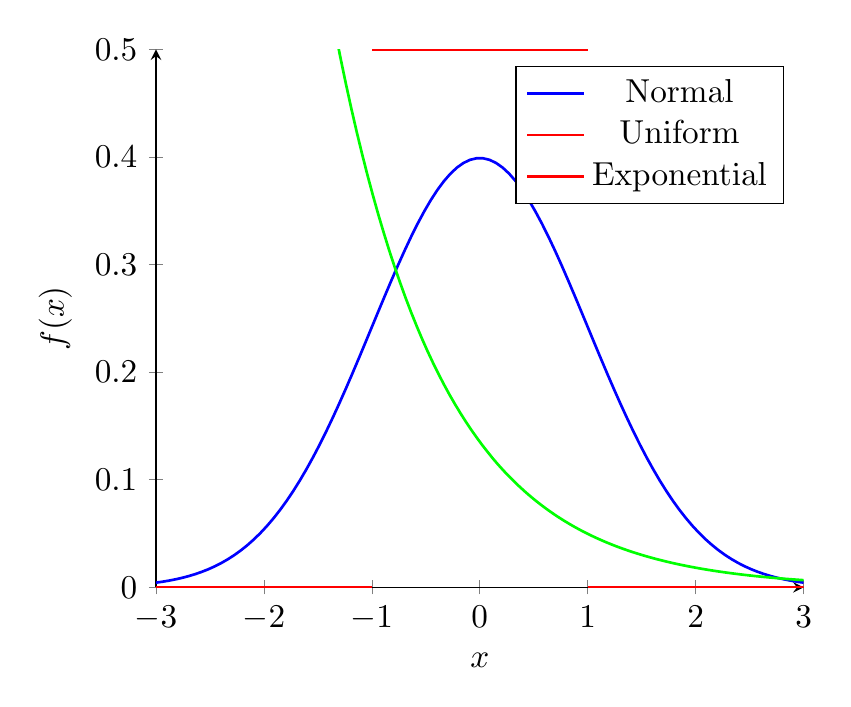
\begin{tikzpicture}[scale=1.2]
    \begin{axis}[
        axis lines = left,
        xlabel = $x$,
        ylabel = $f(x)$,
        xmin=-3, xmax=3,
        ymin=0, ymax=0.5,
        legend pos=north east,
    ]
    
    % Normal distribution
    \addplot[blue, thick, domain=-3:3, samples=100] {exp(-x^2/2)/sqrt(2*pi)};
    \addlegendentry{Normal}
    
    % Uniform distribution
    \addplot[red, thick, domain=-1:1] {0.5};
    \addplot[red, thick] coordinates {(-3,0) (-1,0)};
    \addplot[red, thick] coordinates {(1,0) (3,0)};
    \addlegendentry{Uniform}
    
    % Exponential distribution (shifted)
    \addplot[green, thick, domain=-2:3, samples=100] {exp(-(x+2))};
    \addlegendentry{Exponential}
    
    \end{axis}
\end{tikzpicture}
\caption{Common probability density functions}
\end{figure}

\section{Common Distributions}

\subsection{Discrete Distributions}

\subsubsection{Bernoulli Distribution}
\begin{definition}
$X \sim \text{Bernoulli}(p)$ if $P(X = 1) = p$ and $P(X = 0) = 1-p$.
$$E[X] = p, \quad \text{Var}(X) = p(1-p)$$
\end{definition}

\subsubsection{Binomial Distribution}
\begin{definition}
$X \sim \text{Binomial}(n,p)$ if $P(X = k) = \binom{n}{k} p^k (1-p)^{n-k}$.
$$E[X] = np, \quad \text{Var}(X) = np(1-p)$$
\end{definition}

\subsubsection{Poisson Distribution}
\begin{definition}
$X \sim \text{Poisson}(\lambda)$ if $P(X = k) = \frac{e^{-\lambda} \lambda^k}{k!}$.
$$E[X] = \lambda, \quad \text{Var}(X) = \lambda$$
\end{definition}

\subsection{Continuous Distributions}

\subsubsection{Uniform Distribution}
\begin{definition}
$X \sim \text{Uniform}(a,b)$ has PDF $f(x) = \frac{1}{b-a}$ for $x \in [a,b]$.
$$E[X] = \frac{a+b}{2}, \quad \text{Var}(X) = \frac{(b-a)^2}{12}$$
\end{definition}

\subsubsection{Normal Distribution}
\begin{definition}
$X \sim \mathcal{N}(\mu, \sigma^2)$ has PDF $f(x) = \frac{1}{\sqrt{2\pi\sigma^2}} e^{-\frac{(x-\mu)^2}{2\sigma^2}}$.
$$E[X] = \mu, \quad \text{Var}(X) = \sigma^2$$
\end{definition}

\subsubsection{Exponential Distribution}
\begin{definition}
$X \sim \text{Exponential}(\lambda)$ has PDF $f(x) = \lambda e^{-\lambda x}$ for $x \geq 0$.
$$E[X] = \frac{1}{\lambda}, \quad \text{Var}(X) = \frac{1}{\lambda^2}$$
\end{definition}

\section{Convergence of Random Variables}

\subsection{Almost Sure Convergence}
\begin{definition}
$X_n \to X$ \textbf{almost surely} if $P(\lim_{n \to \infty} X_n = X) = 1$.
\end{definition}

\subsection{Convergence in Probability}
\begin{definition}
$X_n \to X$ \textbf{in probability} if for every $\epsilon > 0$:
$$\lim_{n \to \infty} P(|X_n - X| > \epsilon) = 0$$
\end{definition}

\subsection{Convergence in Distribution}
\begin{definition}
$X_n \to X$ \textbf{in distribution} if $\lim_{n \to \infty} F_{X_n}(x) = F_X(x)$ for all continuity points of $F_X$.
\end{definition}

\subsection{Convergence in $L^p$}
\begin{definition}
$X_n \to X$ \textbf{in $L^p$} if $\lim_{n \to \infty} E[|X_n - X|^p] = 0$.
\end{definition}

\section{Limit Theorems}

\subsection{Law of Large Numbers}
\begin{theorem}[Strong Law of Large Numbers]
If $X_1, X_2, \ldots$ are i.i.d. with $E[X_i] = \mu < \infty$, then:
$$\frac{1}{n} \sum_{i=1}^n X_i \to \mu \text{ almost surely}$$
\end{theorem}

\subsection{Central Limit Theorem}
\begin{theorem}[Central Limit Theorem]
If $X_1, X_2, \ldots$ are i.i.d. with $E[X_i] = \mu$ and $\text{Var}(X_i) = \sigma^2 < \infty$, then:
$$\frac{\sqrt{n}(\bar{X}_n - \mu)}{\sigma} \xrightarrow{d} \mathcal{N}(0,1)$$
\end{theorem}

% Illustration of Central Limit Theorem
\begin{figure}[h]
\centering
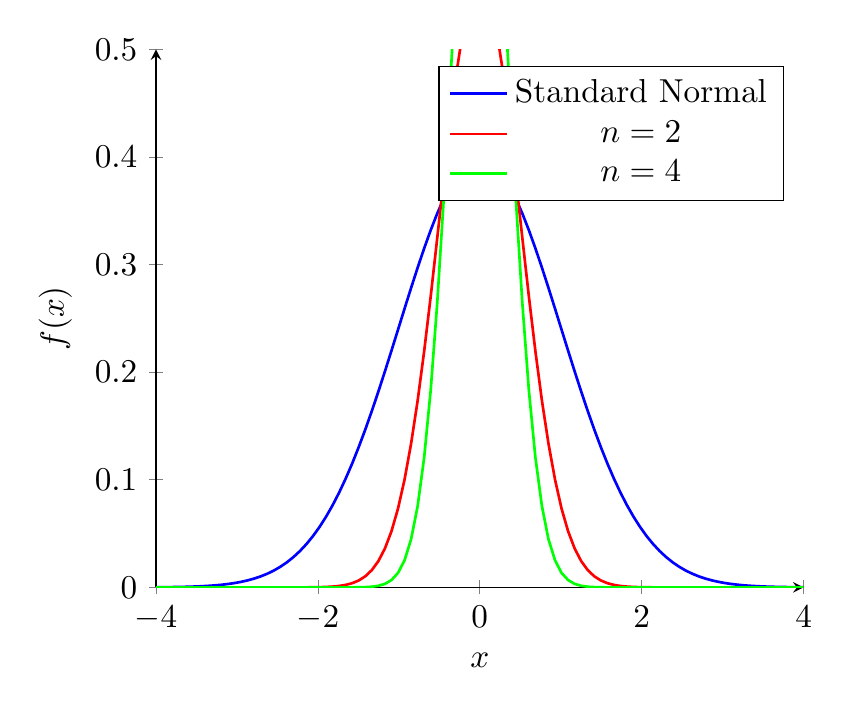
\begin{tikzpicture}[scale=1.2]
    \begin{axis}[
        axis lines = left,
        xlabel = $x$,
        ylabel = $f(x)$,
        xmin=-4, xmax=4,
        ymin=0, ymax=0.5,
        legend pos=north east,
    ]
    
    % Standard normal
    \addplot[blue, thick, domain=-4:4, samples=100] {exp(-x^2/2)/sqrt(2*pi)};
    \addlegendentry{Standard Normal}
    
    % Sample means for different n
    \addplot[red, thick, domain=-4:4, samples=100] {exp(-x^2/0.5)/sqrt(2*pi*0.5)};
    \addlegendentry{$n=2$}
    
    \addplot[green, thick, domain=-4:4, samples=100] {exp(-x^2/0.25)/sqrt(2*pi*0.25)};
    \addlegendentry{$n=4$}
    
    \end{axis}
\end{tikzpicture}
\caption{Central Limit Theorem: convergence of sample means to normal distribution}
\end{figure}

\section{Conditional Probability and Independence}

\subsection{Conditional Probability}
\begin{definition}
The \textbf{conditional probability} of $A$ given $B$ is:
$$P(A|B) = \frac{P(A \cap B)}{P(B)}$$
provided $P(B) > 0$.
\end{definition}

\subsection{Independence}
\begin{definition}
Events $A$ and $B$ are \textbf{independent} if $P(A \cap B) = P(A)P(B)$.
\end{definition}

\subsection{Conditional Expectation}
\begin{definition}
The \textbf{conditional expectation} $E[X|Y]$ is the random variable that equals $E[X|Y=y]$ when $Y=y$.
\end{definition}

\section{Characteristic Functions}

\subsection{Definition}
\begin{definition}
The \textbf{characteristic function} of random variable $X$ is:
$$\phi_X(t) = E[e^{itX}] = \int_{-\infty}^{\infty} e^{itx} \, dF_X(x)$$
\end{definition}

\subsection{Properties}
\begin{theorem}
\begin{enumerate}
    \item $\phi_X(0) = 1$
    \item $|\phi_X(t)| \leq 1$
    \item $\phi_{aX+b}(t) = e^{itb}\phi_X(at)$
    \item If $X$ and $Y$ are independent, then $\phi_{X+Y}(t) = \phi_X(t)\phi_Y(t)$
\end{enumerate}
\end{theorem}

\section{Martingales}

\subsection{Definition}
\begin{definition}
A sequence of random variables $\{X_n\}$ is a \textbf{martingale} with respect to filtration $\{\mathcal{F}_n\}$ if:
\begin{enumerate}
    \item $X_n$ is $\mathcal{F}_n$-measurable
    \item $E[|X_n|] < \infty$
    \item $E[X_{n+1}|\mathcal{F}_n] = X_n$
\end{enumerate}
\end{definition}

\subsection{Martingale Convergence Theorem}
\begin{theorem}
If $\{X_n\}$ is a martingale with $\sup_n E[|X_n|] < \infty$, then $X_n$ converges almost surely.
\end{theorem}

\section{Stochastic Processes}

\subsection{Markov Chains}
\begin{definition}
A \textbf{Markov chain} is a sequence of random variables $\{X_n\}$ such that:
$$P(X_{n+1} = j | X_n = i, X_{n-1} = i_{n-1}, \ldots, X_0 = i_0) = P(X_{n+1} = j | X_n = i)$$
\end{definition}

\subsection{Brownian Motion}
\begin{definition}
\textbf{Brownian motion} $\{B_t\}_{t \geq 0}$ is a stochastic process such that:
\begin{enumerate}
    \item $B_0 = 0$
    \item $B_t - B_s \sim \mathcal{N}(0, t-s)$ for $s < t$
    \item Increments are independent
    \item Paths are continuous
\end{enumerate}
\end{definition}

% Illustration of Brownian motion
\begin{figure}[h]
\centering
\begin{tikzpicture}[scale=1.2]
    \begin{axis}[
        axis lines = left,
        xlabel = $t$,
        ylabel = $B_t$,
        xmin=0, xmax=10,
        ymin=-3, ymax=3,
    ]
    
    % Brownian motion path
    \addplot[blue, thick, mark=none] coordinates {
        (0,0) (1,0.5) (2,-0.2) (3,0.8) (4,0.1) (5,-1.2) (6,-0.5) (7,1.1) (8,0.3) (9,-0.8) (10,0.2)
    };
    
    \end{axis}
\end{tikzpicture}
\caption{Sample path of Brownian motion}
\end{figure}

\section{Applications}

\subsection{Finance}
Probability theory is fundamental to:
\begin{itemize}
    \item Option pricing (Black-Scholes model)
    \item Risk management
    \item Portfolio optimization
    \item Credit risk modeling
\end{itemize}

\subsection{Statistics}
Applications include:
\begin{itemize}
    \item Parameter estimation
    \item Hypothesis testing
    \item Confidence intervals
    \item Bayesian inference
\end{itemize}

\subsection{Physics}
Used in:
\begin{itemize}
    \item Statistical mechanics
    \item Quantum mechanics
    \item Brownian motion
    \item Phase transitions
\end{itemize}

\section{Important Theorems}

\subsection{Radon-Nikodym Theorem}
\begin{theorem}
If $\mu$ and $\nu$ are $\sigma$-finite measures with $\nu \ll \mu$, then there exists a measurable function $f$ such that $\nu(A) = \int_A f \, d\mu$.
\end{theorem}

\subsection{Fubini's Theorem}
\begin{theorem}
If $f$ is integrable on $X \times Y$, then:
$$\int_{X \times Y} f \, d(\mu \times \nu) = \int_X \left(\int_Y f(x,y) \, d\nu(y)\right) d\mu(x)$$
\end{theorem}

\subsection{Dominated Convergence Theorem}
\begin{theorem}
If $f_n \to f$ almost everywhere and $|f_n| \leq g$ for some integrable $g$, then:
$$\lim_{n \to \infty} \int f_n \, d\mu = \int f \, d\mu$$
\end{theorem}

\end{document}
